\documentclass[11pt]{article}
\usepackage{hyperref}
\usepackage{amsmath}
\usepackage{float}
\usepackage[margin=1in]{geometry}
\usepackage{graphicx}
\usepackage{titling}
\usepackage{setspace}

\graphicspath{{../images/}}

\newcommand{\subtitle}[1]{%
  \posttitle{%
    \par\end{center}
    \begin{center}\large#1\end{center}
    \vskip0.5em}%
}

\title{Power Grid Anomaly Detection}
\subtitle{CMPT 318 - Cybersecurity \\ Fall 2021 \\ Uwe Glaesser}

\author{    
    Sajandeep Toor\\
    \texttt{301426579}
    \and 
    Steven Xia\\
    \texttt{301444281}
}

\date{\today}

\begin{document}

\maketitle 
\vspace{5em}

\doublespacing % add double spacing after title

\begin{abstract}
  The threat of cyberattacks is growing rapidly.
  Threats are becoming more complex, sophisticated and difficult to detect. 
  Power grids are vital to the security and health of our society and nation, and 
  are at risk of cyberattacks.
  This project aims to detect anomalies in power grid data using Hidden Markov 
  Models. 
  Preventing cyberattacks on power grids and allow systems or engineers to promptly
  take further action to prevent damage to the power grid.
\end{abstract}

\pagebreak

\singlespacing % remove double spacing for table of contents
\tableofcontents

\pagebreak

\renewcommand{\listfigurename}{Table of Figures}
\listoffigures

\pagebreak

\doublespacing % add double spacing again

\section{Introduction}
With the presence of Advanced Persistent Threats (APTs), Supervisory Control and 
Data Acquisition (SCADA) systems are under attack. 
SCADA systems are used to monitor and control the power grid and other critical 
infrastructure.
Critical infrastructure needs to be monitored autonomously to ensure safe operation
as failure in these systems can lead to catastrophic losses in life.
Increased reliance on automation, means an increased attack surface for APTs.
As power grid operation is crucial; a threat to the power grid is a threat to
security, health and well-being of the people and the nation. 
APTs are a new class of cyber threats, which cannot be detected by traditional 
means of signature based threat detection. 
These threats must be detected by systems that monitor the power grid and 
detected anomalies in the power grid's behaviour and take appropriate actions 
promptly.
This is where anomaly detection and Hidden Markov Models (HMMs) come in.
This report takes a look at the power grid anomaly detection using HMMs.

  \subsection{Threats to Cybersecurity} 
  The importance of cybersecurity is crucial, the number of threats and damage 
  done to digital systems and infrastructure is growing rapidly each year. 
  Threats themselves are evolving, becoming more severe, common, and difficult to 
  detect.
  The average ransom payments have gone up more than 14 times from Q3 of 2018 to
  Q1 of 2020, from around \$10,000 to \$140,000.
  This shows a significant increase in the severity, frequency and cost of cyber 
  threats.
  Growth of Internet connected devices is similar, growing through the Internet of 
  Things (IoT). 
  Experts are expecting to have 22 billion IoT devices by 2025.
  This makes cybersecurity even more important as IoT devices can form botnets, 
  powering DDoS attacks such as Mirai. 
  APTs are a new class of cyber threats, where the goal is to remain undetected
  for as long as possible, understand the system, and place malicious code on the 
  system.
  These threats can only be detected by anomaly detection methods, not by 
  traditional means of cybersecurity.


\section{Anomaly Detection}
What is an anomaly? Anomalies are events that do not conform to normal behaviour. 
To understand an anomaly, we must understand the normal behaviour of the system.  
There are three types of anomalies: 
  \begin{itemize}
    \item Point Anomalies: The simplest type of anomaly, these are data points that 
    are outside the normal distribution of the data.
    \item Contextual Anomalies: Anomalies in specific context. For example, snow 
    in the middle of summer would be anomalous, but the event of snowing itself 
    is not anomalous.
    \item Collective Anomalies: Anomalies that are not anomalous themselves, but 
    together are anomalous. For example, an irregular heartbeat pattern.
  \end{itemize}

  We focus on collective anomalies in our HMM implementation of anomaly detection.

  \subsection{Hidden Markov Models and Anomaly Detection}
  Hidden Markov Models (HMMs) are a key tool in anomaly detection.
  HMMs allow us to model the normal behaviour of a system provided we have a 
  dataset with normal behaviour or mostly normal behaviour. 
  Once we have a properly trained model, i.e. representing normal behaviour, we 
  can use the model to detect anomalies. 

  \subsection{Fitting of a Model}
  What is a properly fitted model?  
  To understand properly fitting of a model, it is required to understand badly
  fitted models.
  There are two types of badly fitted models, overfitted and underfitted models.
  Overfitting is where the model produces a strong fit to the training data 
  but does poorly on testing data.
  This is because the model is fitted to the noise of the training data and 
  ``thinks'' that is the representation of normal behaviour.
  Overfitting can be caused by having too many states in the model, selecting 
  too many features or selecting features that are too correlated to each other, thus 
  having redundancy in their data.
  The opposite problem is underfitting, where the model produces a poor fit to the
  training data and testing data.
  This means the model is not able to represent the normal behaviour.
  Underfitting can be caused by having too few states in the model, selecting
  too few features or not having enough data to train the model.

\section{Methodology}
  \subsection{Data Analysis}
  The power grid time series dataset is from December 16\textsuperscript{th}, 2006 to December
  1\textsuperscript{st} 2009, approximately 3 years of power grid data. 
  The dataset has values for several characteristics or features, global active power, global
  reactive power, global intensity, voltage and sub metering 1 to 3. 
  Some of this information is more relevant to the anomaly detection problem than others. 
  This will be discussed in detail in \textbf{Feature Engineering}.
  The interval we selected was Wednesday, 6PM to 9PM. 

    \subsubsection{Data Cleaning and Scaling}
    The data was broken up into each observation, an observation being a measurement of the power
    grid features, which happened every minute.
    A problem we noticed with this dataset is it had a lot of missing values. 
    To solve this problem, the data had to be processed and cleaned.
    Two methods were used to remove the missing values: if a group of missing values was less than
    five minutes long, it was linearly interpolated, otherwise, the entire time interval was
    removed.
    This was because long time intervals cannot be accurately enough interpolated and would result
    in a worse performance in training.
    However, the short missing values were interpolated to maximize the amount of data we had
    access to.

    The data also had to be scaled, the scaling was done using Python with the
    \texttt{StandardScaler} class from the \texttt{sklearn} library.
    This class standardizes the features of the data meaning the values of the data set are made to
    have a mean of zero and unit standard deviation. 
    We chose to scale with standardization rather than normalization because it is more lenient
    with regard to noise as it does not force concrete minimal and maximal values to the data,
    overly scaling the ``useful'' portions of the data to a tiny range.
    This would be a major problem with noisy data. 

   \subsection{Feature Engineering}
    Feature engineering is the process of selecting features from the data to use in our model.
    This step is incredibly important because, as is discussed later, it may make or break the
    effectiveness of our model.
    Selecting too few features will result in a dataset that is not representative of the
    behaviour of the system, which will result in underfitting.
    On the other hand, if too many features are selected, we will run the risk of overfitting.
    To avoid overfitting, we must select a small subset of features.
    Furthermore, it would be best to select features that are not correlated to each other as
    correlation between features increases the risk of overfitting.
    To determine which features to use, we used \textbf{Principal Component Analysis}.

    \subsubsection{Principal Component Analysis}
    Principal Component Analysis (PCA) is a statistical method allowing us to see the correlation
    between features in the data.
    PCA was originally designed to be a dimensionality reduction algorithm, something used to
    reduce the number of features in a dataset while keeping most of the variance.
    However, we can also use it to determine which features are most important by looking at only
    the first few principal components that it calculates, and seeing which of the features factor
    into those components.
    This allows us to select multiple features that do not contain redundant information, lowering
    chance of overfitting our model.

    \subsection{Training Models}
    We split the interval data into training and testing datasets.
    The training dataset contained the first 66.66\% of the intervals in the data, while the
    test dataset contained the last 33.33\% of the intervals in the data.
    Since the dataset contains observations spanning approximately three years, 
    this means the training data consists of mostly the first two years while the testing data contains the last year.
    To train our model, we used the R package \texttt{depmixS4}.
    This allowed us to train HMMs using the \texttt{depmix} function.

    A problem was selecting the number of states and the distribution family of our data. 
    The distribution family chosen for both our features was the Gaussian distribution.
    Increasing the number of states in the model would increase the complexity of the model,
    risking overfitting, while decreasing the number of states would result in an underfitted
    model.
    Because of this, we wrote a script that tested every number of states in the range 4–24 and
    plotted their train and test log-likelihoods on a graph to illustrate if there was any
    overfitting that was occurring.

    \subsection{Testing Models}
    Testing the model is crucial; we must confirm that our model understands what normal behaviour
    looks like and confirm that it is fitted properly. 
    Testing involves feeding the model data that it has not seen before and seeing whether the
    log-likelihood value on that data is reasonably close to the training data.
    If the likelihood is low, then the model is not properly fitted, therefore, our final model was
    the one with the highest log-likelihood on the test data.

  \subsection{Anomaly Detection in Power Grid}
  After training, testing and picking the best possible model, we have a model that
  represents normal behaviour. 
  As anomalies are events that deviate from normal behaviour, we can use this model to detect
  anomalies in the stream data.
  Our data with anomalies was processed and scaled in the same way as our training and testing data.
  From there, we break the data with anomalies into each interval and feed it into the model
  representing normal behaviour.
  If the log-likelihood is lower than some threshold, then there seems to be an anomaly in the
  interval according to the model. 
  This would be a collective anomaly.
  On the other hand, if the log-likelihood is higher than that threshold, then there is no anomaly
  in the interval and the observation represents normal behaviour. 

  \subsection{Point Anomaly Detection}
  Our approach with HMMs for anomaly detection captures collective anomalies, rather 
  than point anomalies. 
  If we want to detected point anomalies, we would have to take a different approach.
  For point anomalies we used the scaled data mentioned in \textbf{Data Cleaning and Scaling},
  then from all intervals in the data, we take the average value at each minute 
  for each feature we selected in \textbf{Feature Engineering}.
  This would represent the average normal behaviour of the power grid for our chosen interval.
  As we know the testing dataset has mostly no anomalies, we can find thresholds 
  for each feature that minimizes the amount of point anomalies in the testing dataset.
  Since it is not guaranteed that the testing dataset has no anomalies, we must make a 
  guess for the amount of anomalies in the testing dataset.
  Then, we compute the difference between the values of the average observation 
  and the anomaly observation for each feature and see if it is greater than the computed 
  thresholds to determine whether the point is anomalous or not.

\section{Results}

\subsection{Principal Component Analysis}
\begin{figure}[H]
  \centering
  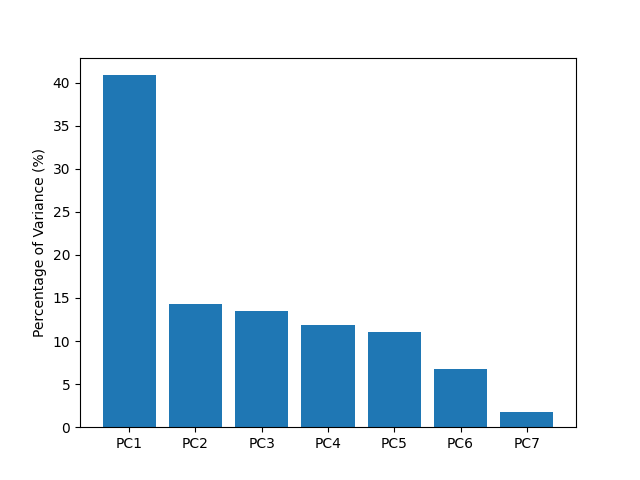
\includegraphics[scale=0.7, trim=15 20 30 40, clip]{../images/PCA_Variance.png}
  \caption{PCA: Variance of Project Data}
\end{figure}

From Figure 1, the first component, PC1 holds about 41\% of the data, while 
the rest of the components hold less than 15\% of the data each.
This makes PC1 the most important component to explain the variance of the data.

\begin{figure}[H]
  \centering
  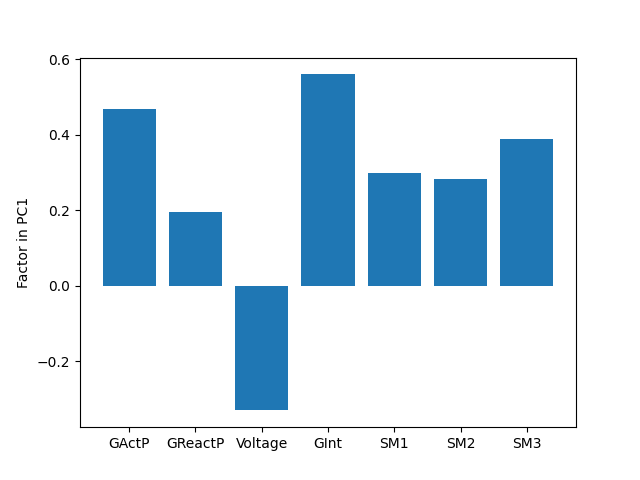
\includegraphics[scale=0.7, trim=0 0 15 20, clip]{../images/PC1_Factors.png}
  \caption{Variance of each feature in PC1}
\end{figure}

Figure 2 depicts the variance of each feature in PC1.
The most important feature, GInt or Global Intensity, represents about 56\% of 
the variance in PC1. 
The second most important feature is GActP or Global Active Power, which represents 
about 47\% of the variance in PC1.
Some other notable features are voltage, and SM3 or Sub Metering 3. 
However, these features do not represent as much of the variance in PC1.

\begin{figure}[H]
  \centering
  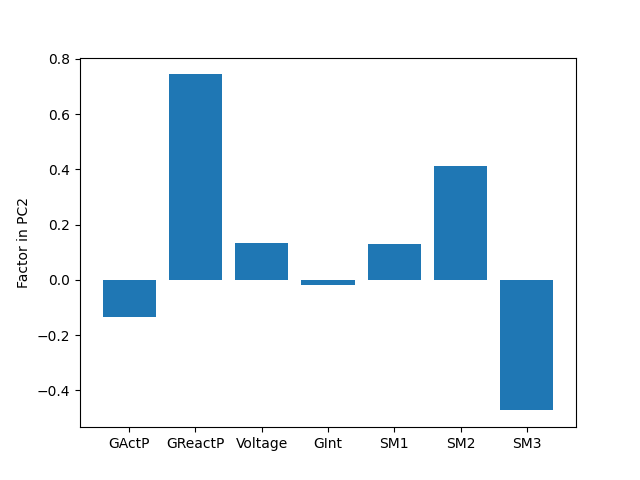
\includegraphics[scale=0.7, trim=0 0 15 20, clip]{../images/PC2_Factors.png}
  \caption{Variance of each feature in PC2}
\end{figure}

Figure 3 depicts the variance of each feature in PC2.
The most important feature is GReactP or Global Reactive Power, which represents
about 74\% of the variance in PC2.
The second most important feature is SM3 or Sub Metering 3, which represents
about 41\% of the variance in PC2.
Although PC2, holds a little under 15\% of the total variance in the data, it also
helps us with feature engineering. 

\begin{figure}[H]
  \begin{minipage}{0.499\textwidth}
    \centering
    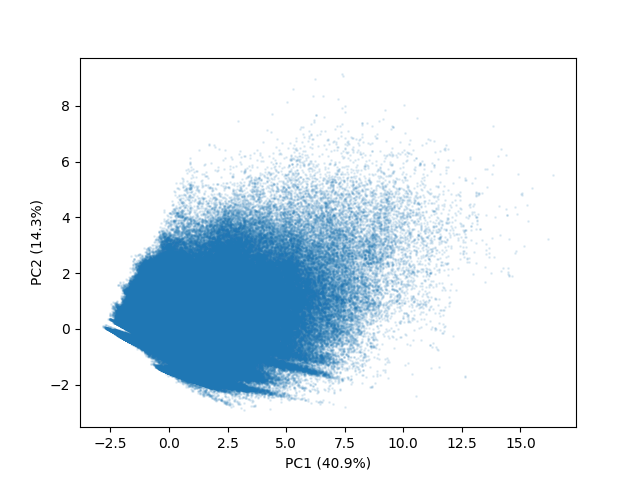
\includegraphics[width=\textwidth, trim=0 0 30 40, clip]{../images/PC1_PC2.png}
    \caption{PCA Graph: PC1 vs PC2}
  \end{minipage}\hfill
  \begin{minipage}{0.499\textwidth}
    \centering
    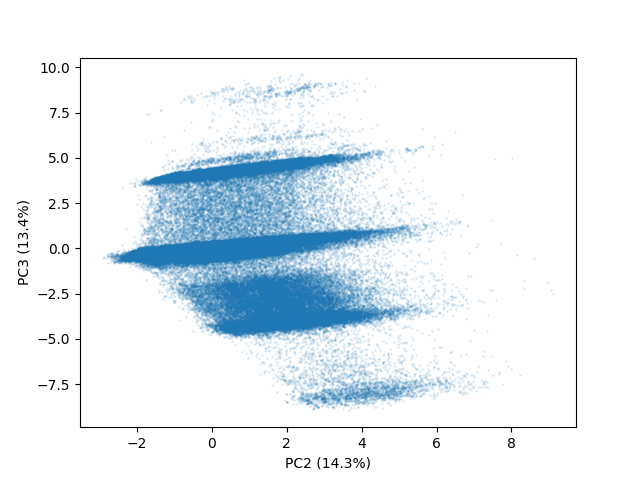
\includegraphics[width=\textwidth, trim=0 0 30 40, clip]{../images/PC2_PC3.png}
    \caption{PCA Graph: PC2 vs PC3}
  \end{minipage}
\end{figure}

Based off the results of our Principal Component Analysis, the features we chose 
to use for our model were Global Active Power and Global Intensity.
Although Sub Metering 3 could be argued to be an important feature as well, we 
choose not to use as choosing too many features could result in overfitting.

\subsection{Training \& Testing} 

\begin{figure}[H]
  \centering
  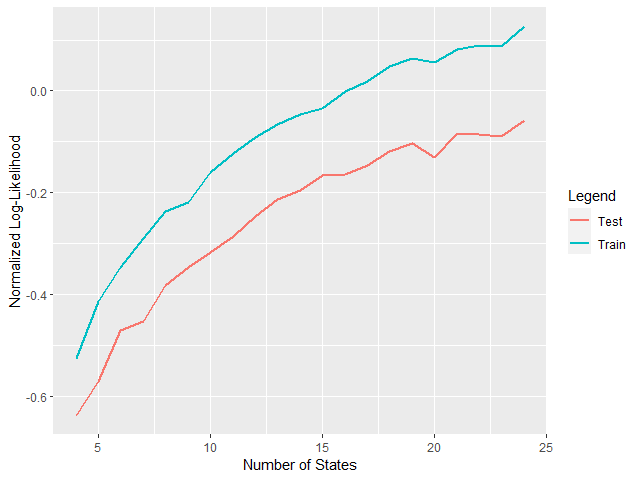
\includegraphics[scale=0.7]{../images/TrainTest.png}
  \caption{Log-likelihood of Training and Testing Data}
\end{figure}

Figure 6 shows that increasing the number of states of the HMM, increased the 
log-likelihood of the model in training and testing. 
The testing log-likelihood was consistently a little under the training log 
likelihood, which is what we expected and does not show any signs of overfitting.

\begin{figure}[H]
  \centering
  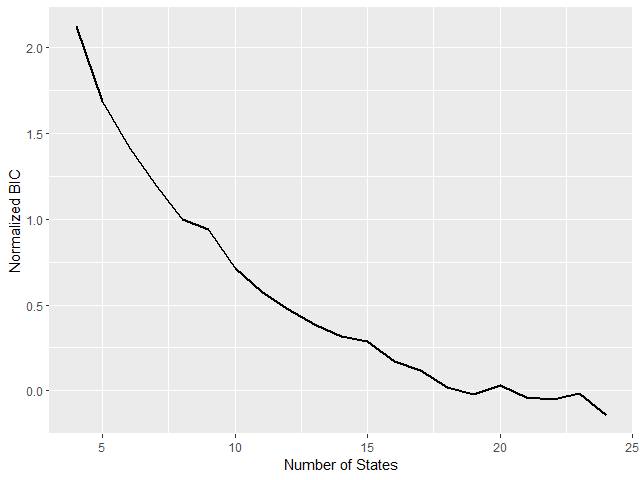
\includegraphics[scale=0.7]{../images/ModelBIC.png}
  \caption{Normalized BIC of Training}
\end{figure}

Figure 7 shows the normalized Bayesian Information Criterion (BIC) values of 
training the HMMs with different number of states.
The BIC values decrease with the increasing number of states, showing that 
despite increasing the complexity of the model with more states, the model does 
not overfit the training data.

From our results, we found the best HMM is the one with 24 states where the 
log-likelihood for testing data was maximized and BIC values were minimized.

\subsection{Anomaly Detection}

\begin{figure}[H]
  \centering
  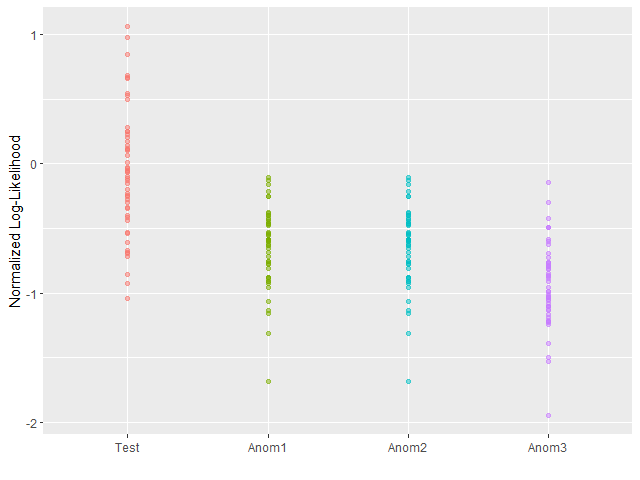
\includegraphics[scale=0.7]{../images/IndividualLogLike.png}
  \caption{Normalized log-likelihood of Individual Interval in Testing and Anomaly Data}
\end{figure}

Figure 8 shows the log-likelihood of each interval in the testing and anomaly data. 
The normalized log-likelihood of testing data was generally higher than the 
normalized log-likelihood of anomaly data, which is what we expected. 
This is because the testing data is representation of normal behaviour. 
The normalized log-likelihood of the anomaly dataset was lower with several 
outliers, showing potential anomalies in the data. 
This shows that our HMM has a good understanding of normal behaviour in the data,
allowing us to detect anomalies.

\subsection{Point Anomaly Detection}
For point anomaly detection, we guessed about 50 point anomalies in our testing 
dataset.
This can be argued to be too little for a dataset with 9000 points, 
but we see that this value is able to detect a significant amount of
point anomalies.
Also, in the context of power grid, too many false positives can be a massive problem 
and an annoyance to everyone.
For each of our features, Global Active Power and Global Intensity, we computed
the thresholds using testing data.
We found that the maximum and minimum thresholds for Global Active Power were \texttt{5.06566} and \texttt{-4.00648} respectively.
For Global Intensity, we found that the maximum and minimum thresholds were \texttt{15.5016} 
and \texttt{-17.1333}. 

Using these thresholds, we found the number of point anomalies in anomaly datasets 1, 
2 and 3 were \texttt{47}, \texttt{47}, and \texttt{2530} respectively.
There were a significant amount of point anomalies in anomaly dataset 3, and anomaly 
dataset 3 was the most anomalous dataset, showing that our approach for point anomaly 
detection is a good approach.

\section{Conclusion}

\subsection{Accomplishments}
The result of this project is a Hidden Markov Model that is able to predict, to a degree, whether
there is an anomaly in certain power grid statistics. This can in turn alert the supervisory
control system, or the human engineers, of the issue and allow them to take appropriate action.

The log-likelihood threshold of determining an anomaly should be tweaked depending on the specific
use case of the model and is beyond the scope of this project.
Similarly, the number of point anomalies in the test dataset should also be adjusted.
However, as a demonstration, if we assume that the cost of a false positive and a false negative
are equivalent and also happen equally as often, the optimal log-likelihood threshold is 
\texttt{-0.342}
which results in a false positive rate of \texttt{25.5\%} and a false negative rate of \texttt{9.3\%}
Within the source code of this project is a script that can calculate the optimal threshold given
the ratio of frequencies of normal to anomalous behaviour, and the ratio of costs of a false
negative to a false positive.

\subsection{Challenges}
A major challenge to the deployment of the trained model is that there is still a substantial
amount of overlap between the log-likelihoods of individual intervals from the testing data set and
the anomaly data set (as seen in Figure 8).
As such, there is no static threshold that can be able to detect an anomaly with absolute
certainty.
Considering this, determining the ``proper'' threshold for detecting anomalies will depend on the
result of a risk assessment report, with which we can use to calculate the optimal threshold to
minimize potential damages.

Another challenge was a lack of ground truth in the provided data. 
We did not know if there were any anomalies in our data, what kind of anomalies they were, etc. 
We made assumptions that the data had ``mostly'' no anomalies, and this could easily be incorrect.
The data also lacked labels for differentiating between normal and anomalous behaviour.

\subsection{Lessons Learned}
There were multiple lessons that were learned during the completion of this project.
The first occurred during the selection of features with which to train the model.
Despite ending up using two features, models trained on one or three features were also
experimented with, however, they both resulted in worse performance than the model trained on two
features.
This confirmed the prior belief that more features did not necessarily result in improved
performance, and also showed that there is often a thin line between providing not enough data and
providing too much of it.

Another thing was learned during the splitting of data into train and test data sets.
Initially, the data was first shuffled before splitting.
This was done with the intention of removing bias that may be caused from different segments of the
data set coming from different times.
However, after stepping back and pondering that decision, we realized that the bias is exactly what
is wanted to simulate the real life scenario that this model will be used in.
The electricity usage changes over time depending on people's habits, and the model will have to be
able to correctly identify anomalies in data sets that have slightly different behaviours than it
is trained on.

\pagebreak

\phantomsection 
\addcontentsline{toc}{section}{Bibliography} 

\begin{thebibliography}{9}

  \bibitem{cyberthreat}
  Canadian Centre for Cyber Security. National Cyber Threat Assessment 2020. 
  Communications Security Establishment, Government of Canada, 2020.

  \bibitem{whatisiot}
  Oracle. \textit{What is the internet of things (IOT)?} | 
  Retrieved December 3, 2021, from https://www.oracle.com/ca-en/internet-of-things/what-is-iot/. 
\end{thebibliography}

\end{document}
